\section{System Architecture}
\label{sec:architecture}

The FlashBoost architecture is a homogeneous cluster of host servers coupled
with a FlashBoost storage device. Each FlashBoost storage device is plugged into
the host server via a PCIe link, and it consists of flash storage, an in-storage
processing engine, 8 high-speed network interfaces and on-board DRAM. The host
servers are networked together using Ethernet or other general-purpose
networking fabric. The host server can access the FlashBoost storage device via
a host interface implemented over PCIe. It can either directly communicate with
the flash interface, to treat is as a raw storage device, or with the in-store
processor to perform computation on the data.

The in-store processing engine has access to four major services: The flash
controller, network controller, host interface and the DRAM Buffer.
Figure~\ref{fig:ispservice} shows the four services. 


\begin{figure}[h]
	\begin{center}
	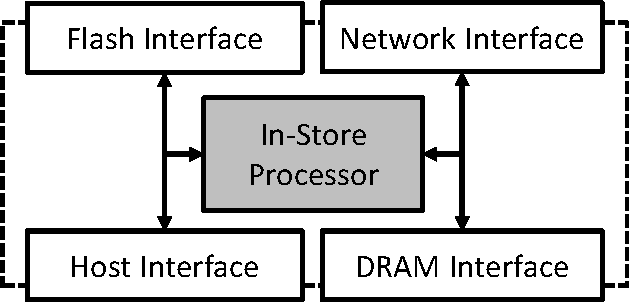
\includegraphics[width=0.3\paperwidth]{figures/isp-service-crop.pdf}
	\caption{Services Provided to In-Store Processor}
	\label{fig:ispservice}
	\end{center}
\end{figure}

In our implementation of FlashBoost, we have used a Field Programmable Gate
Array (FPGA) to implement the in-store processor and also the flash, host and
network controllers. However, the FlashBoost Architecture should not be limited
to an FPGA-based implementation.  Development of FlashBoost was done in the
high-level hardware description language Bluespec. As a result, all services
expose a high-level language interface using latency-insensitive FIFOs for
communication. This makes the services intuitive to use, and flexible to be used
easily with many in-storage processing engines.

\begin{figure*}[ht]
	\begin{center}
	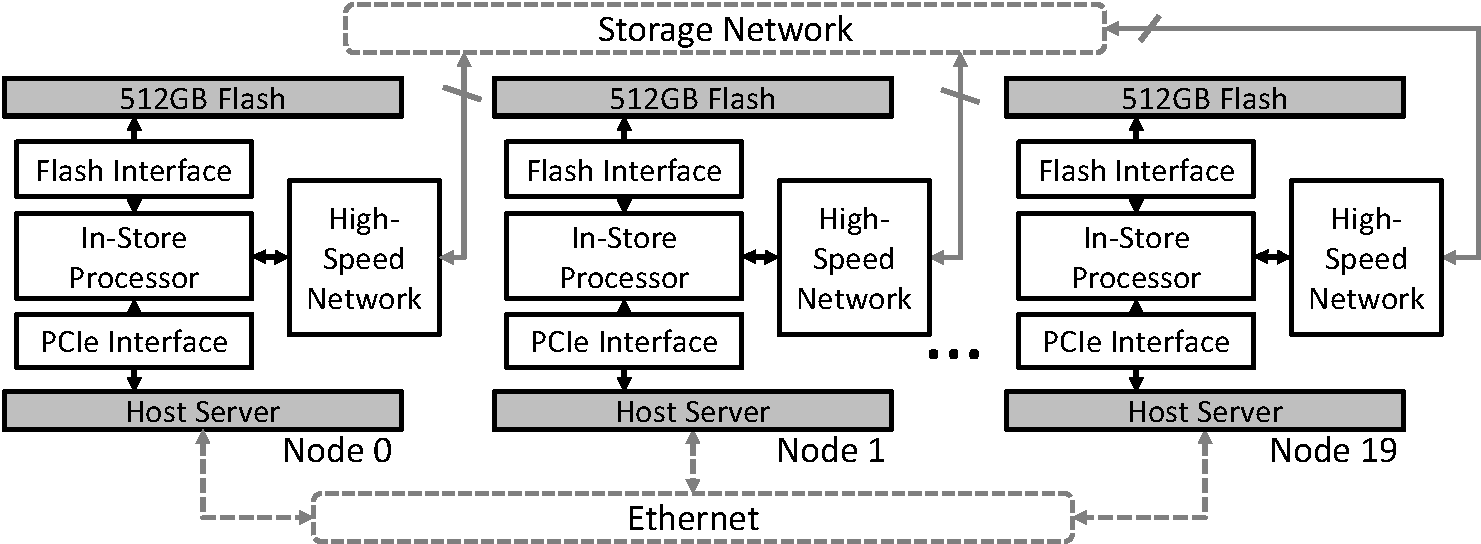
\includegraphics[width=0.8\paperwidth]{figures/architecture.pdf}
	\caption{FlashBoost Architecture}
	\label{fig:architecture}
	\end{center}
\end{figure*}

\subsection{Flash Interface}

Access to flash storage is provided by the flash controller via a
fast, low-level and error-free interface with minimal bandwidth and
latency overhead. This interface exposes the internal memory organization of
the flash device, namely the buses/channels, chips, blocks and pages.
The interface is designed to stream data in
and out of the flash chips as fast as possible without concern for
flash management. Garbage collection, bad block management and
wear-leveling functionalities are handled by the flash-aware file system
in the host kernel (discussed in Section~\ref{sec:software}). The key advantage of such
a low-level interface is that in-store processors have direct access to
the data in a streaming fashion with minimal buffering and insignificant
latency overhead. 

The raw flash interface, in hardware, is defined below:

%[captionpos=b, caption={Flash Controller Interface}, label={lst:hwifc}]
\begin{lstlisting}
interface FlashIfc;       
  method sendCmd (FlashOp op, Bit#(4) bus,
                  Bit#(3) chip, Bit#(16) block, 
                  Bit#(8) page, Bit#(8) tag);        
  method writeWord (Bit#(128) data, Bit#(8) tag);
  method Tuple2#(Bit#(128), Bit#(8)) readWord (); 
  method Bit#(8) writeDataReq ();
  method Tuple2#(Bit#(8), StatusT) ackStatus ();
endinterface 
\end{lstlisting}

To access the flash, the user issues a flash command
(\textit{sendCmd} method) with the operation, the address and
a free tag. For writes, the user awaits for a write data request from
the controller scheduler (\textit{writeDataReq} method), and then sends
the write data corresponding to that request in 128-bit bursts
(\textit{writeWord} method). An acknowledgement is received when the
operation completes (\textit{ackStatus} method). For read operations,
data will return in 128-bit bursts along with the command tag that the
burst corresponds to. We emphasize that for maximum performance, the
controller sends these data bursts \textbf{out of order} with respect to
the issued request and \textbf{interleaved} with other read requests.
Thus completion buffers may be required on the user side. Furthermore,
we note that to saturate the bandwidth of the flash device, multiple
commands must be in-flight at the same time, since flash operations
have latencies of tens to thousands of microseconds. 

In our architecture, multiple users may need shared access to the
flash controller interface. For example, a particular flash controller may
be accessed by local in-store processors, local host software over PCIe
DMA, or remote in-store processors. Thus, we include as part of the
platform, an interface multiplexer that converts one flash interface
into a parametrizable number of additional interfaces. 

%TODO: give a name to this module?
To ease development of hardware accelerators (i.e. in-store processors),
we also provide a parametrizable module that converts a flash interface
into multiple simple in-order request/response interfaces
(Figure~\ref{?}). We allow the user to adjust the interface width, the
command queue depth and number of interfaces of the converter.
Internally, the converter renames tags and uses completion buffers to
order data. This design easily permits multiple accelerators to be
attached to the flash device, taking advantage of flash parallelism. 


\begin{figure}[h]
	\begin{center}
	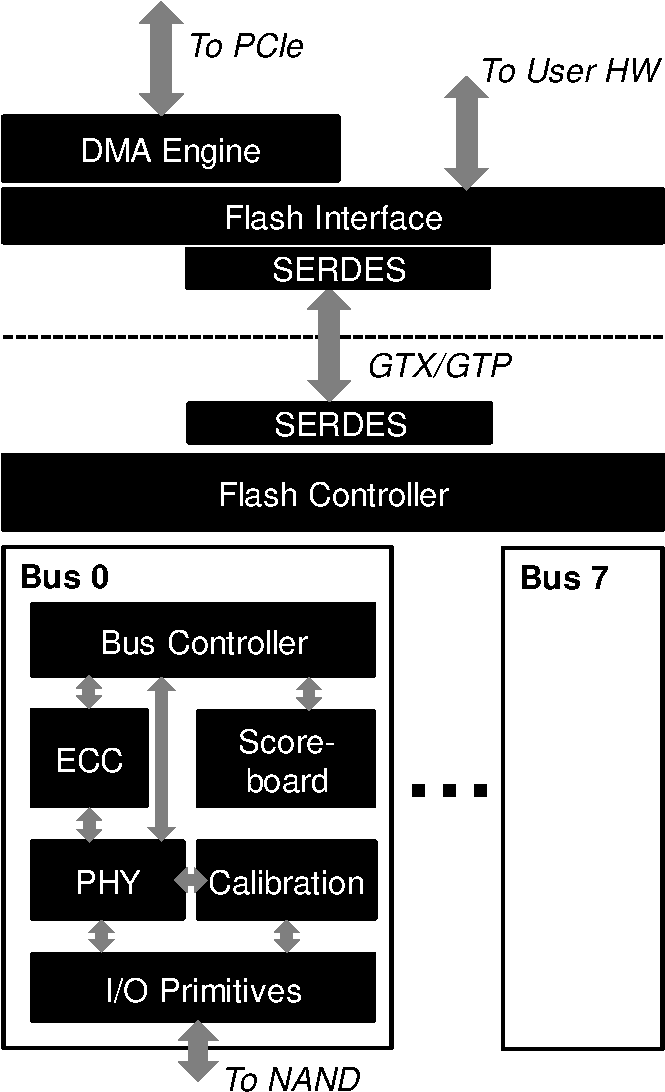
\includegraphics[scale=0.4]{figures/top-arch-crop.pdf}
	\caption{Flash Interface}
	\label{fig:flashinterface}
	\end{center}
\end{figure}

\subsection{Inter-Storage Network}

FlashBoost provides an intuitive network infrastructure across all FlashBoost
storage devices in the cluster.
FlashBoost storage devices are linked among themselves via
high-performance serial links that are separate from the host server network. 
Each storage device has multiple network ports, and acts both as a network switch as
well as a network client. The storage network is implemented entirely inside the
FPGA, and provides very simple functionality such as routing, flow control and
virtual channels to maintain an extremely low latency.

\subsubsection{Network Endpoint}

Each virtual channel is implemented as a pair of send and receive FIFOs that can
be used to send and receive data to and from any node. The programmer can define
multiple virtual channels of arbitrary datatype, and the network infrastructure
serializes and schedules each link onto the network link. These send and receive
FIFOs act like normal FIFOs in that it provides back pressure across the
network. Such intuitive characteristics of the network ease in-storage processor
development.

\begin{verbatim}
NetworkEndpoint#(type Bit#(64)) endpoint1 
     <- mkNetworkEndpoint(1); // endpoint id: 1
NetworkEndpoint#(type Bit#(256)) endpoint2 
     <- mkNetworkEndpoint(8); // endpoint id: 8
List endpoints = 
     cons(endpoint1, cons(endpoint2, nil));
NetworkArbiter arbiter 
     <- mkNetworkArbiter(endpoints);

...
endpoint1.send(data,dest);

...
tuple(data,src) <- endpoint1.receive;
\end{verbatim}

In our FlashBoost implementation, this network is implemented over the
low-latency serial transceivers that are already included in the FPGA. By
implementing routing in the hardware and using a very low-latency network
fabric, we were able to achieve very high performance, with 0.5$\mu s$ of
latency per network hop, and near 10Gbps of bandwidth per link. Our
implementation has a network fan-out of 8 ports per storage node, so the
aggregate network bandwidth available to a node reaches up to 8GB/s, including
packet overhead.

\subsubsection{Link Layer}

The link layer managed physical connections between network ports in the storage
nodes. The most important aspect of the link layer is the simple token-based
flow control implementation. This assures that no packet will drop if the data
rate is higher than what the network can manage, or if the data is not received
from the destination node quick enough.

\subsubsection{Routing Layer}

Figure~\ref{fig:networkinterface} shows the implementation of the router in each
storage node. Each packet can either come from the network port's link layer
interface, or from the user's network endpoint. Each incoming packet's
destination field is compared to the routing table in the router to determine
whether to be forwarded to a remote node via a network port, or to be delivered
to a local endpoint if its destination is the current node. It then goes through
one of the four crossbar switches to be delivered to the correct destination. 
Fairness is implemented using a round-robin priority ordering to ensure maximum
throughput while ensuring no port starves.

It is important to note that the routing table can have more than one network
port entry per destination node index. This is because each pair of nodes can
have more than one immediate link connecting between them, and there may be
multiple viable paths between a pair of two remote nodes. In order to make
maximum use of the available bandwidth in such cases, the routing table can have
entries for multiple valid ports for the next hop. In order to ensure in-order
arrival, the endpoint id of the origin endpoint is hashed to deterministically
decide which entry to use in the routing table. In-order arrival is desirable in
a hardware implementation because completion buffers may be expensive.
Because of this characteristic, if the in-storage processing engine want to
ensure more bandwidth, it can break a wide data bus into multiple endpoints and
send data over them in parallel. Figure~\ref{fig:networkrouting} shows packet
routing in an example network.

\begin{figure}[h]
	\begin{center}
	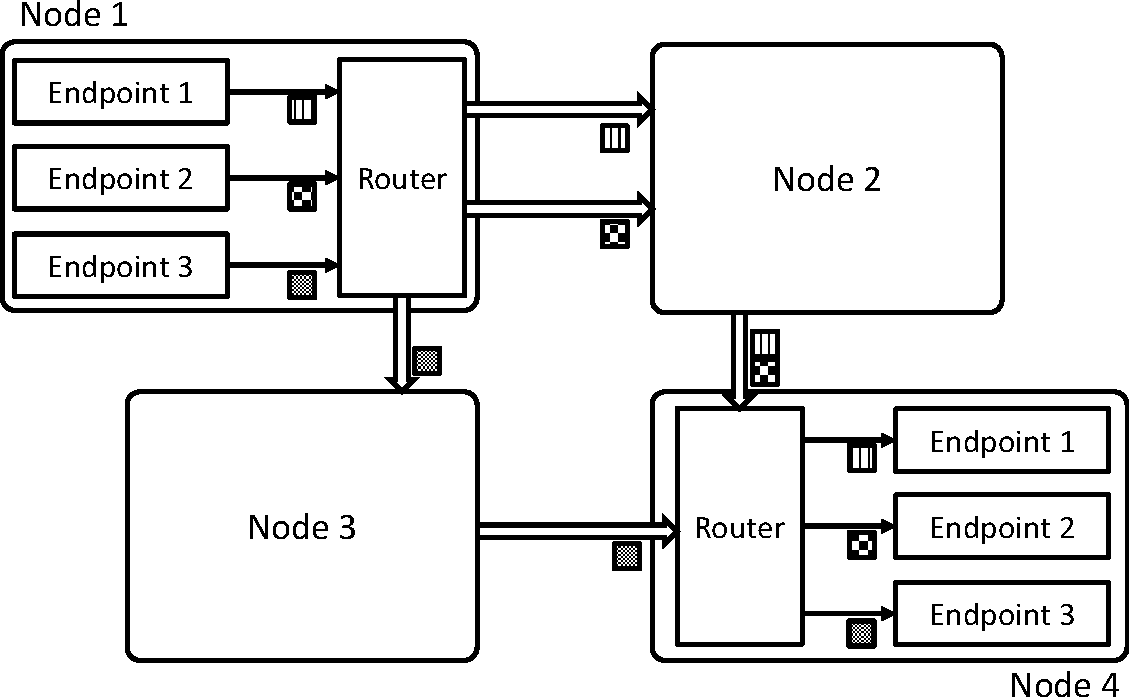
\includegraphics[width=0.4\textwidth]{figures/routing-crop.pdf}
	\caption{Routing Packets Across the Network}
	\label{fig:networkrouting}
	\end{center}
\end{figure}

It should be noted that the infrastructure does not assure that the receiving
side will always be able to receive the data being transferred. If a
destination endpoint is unable to receive data at a fast enough rate, it might
result in related parts of the network being blocked. This was an intentional
design choice to build an extremely low-latency network while maintaining low
resource usage. The programmer can choose to use our provided end-to-end flow
control module on top of the network infrastructure to ensure the data source
will only send data that the receiver have space for, but this results higher
network latency as flow control packets frequently needs to be sent to ensure
free space on the receiving end. This is exacerbated by the fact that memory
resource for large buffers is scarce on the FPGA hardware. On the other hand,
If the designer is sure that the packets will
always be consumed, such additional code can be omitted. 

\begin{figure}[h]
	\begin{center}
	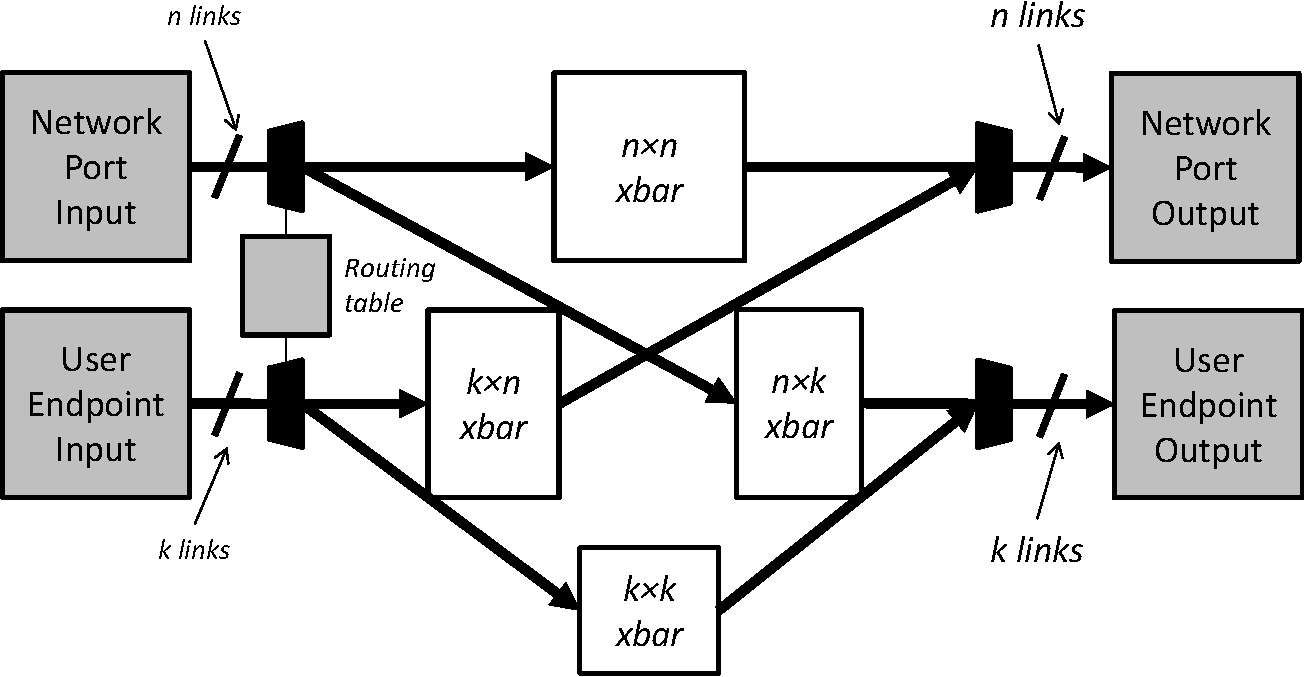
\includegraphics[scale=0.4]{figures/network-routing-crop.pdf}
	\caption{Network Interface}
	\label{fig:networkinterface}
	\end{center}
\end{figure}


\subsection{Host Interface}

The near-data processing core can be accessed from the host server over either a
low-level RPC-like interface or a file system abstraction. Our host interface
was implemented using Connectal~\ref{connectal}, a hardware-software codesign
framework built by Quanta Research Cambridge. Connectal reads the interface
definition file written by the programmer and generates glue logic between
hardware and software. Connectal automatically generates RPC-like interface from
developer-provided interface specification, as well as a
memory-mapped DMA interface for high bandwidth data transfer. Connectal provides
a PCIe Gen 1 endpoint and driver pair, and provides up to 1.6GB/s DMA read to
host DRAM bandwidth and 1GB/s of DMA write from host DRAM bandwidth. 

The software maintains two 128-page page buffers, each for reads and writes. When
issuing a read or write request, the software sends the target or source page
buffer index along with the request to let the hardware side host interface know
where to read or write data from. Since this buffer is returned to the free list
when each operation is finished, the buffer index effectively acts as the locally
unique tag for each flash operation. Writing data is straightforward, as data is
read in-order from the host page buffer and written in-order to each flash
controller bus. 
However, reading from flash is more complex because there is only a single data
bus that connects to the flash interface, and data from different buses can
arrive interleaved. This problem becomes even more
difficult when a node is requesting data from multiple remote nodes, where 
data corresponding to all requests in flight can arrive interleaved with each
other. The naive way to fix this would be to have a FIFO for each possible
tag, so that enough data for a DMA burst can be collected for each tag before
starting a burst. However, this would be an inefficient use of FPGA memory
resources.
To fix this issue, we provide an implementation of a vector of FIFOs implemented
in a single contiguous BRAM block, with BRAM support.

Reading or writing data from the host buffers were done by DMA read/write
engines implemented in the Connectal framework. In our FlashBoost
implementation, there are four read engines and four write engines each, in
order to more easily make maximum use of the PCIe bandwidth. Since there are 16
buses in total per storage node, each read/write engines manage data from four
buses each. Figure~\ref{fig:hostinterface} describes the structure of the host
interface.

\begin{figure}[ht!]
	\centering
%	\subfloat[Writing Data to Storage]
%		{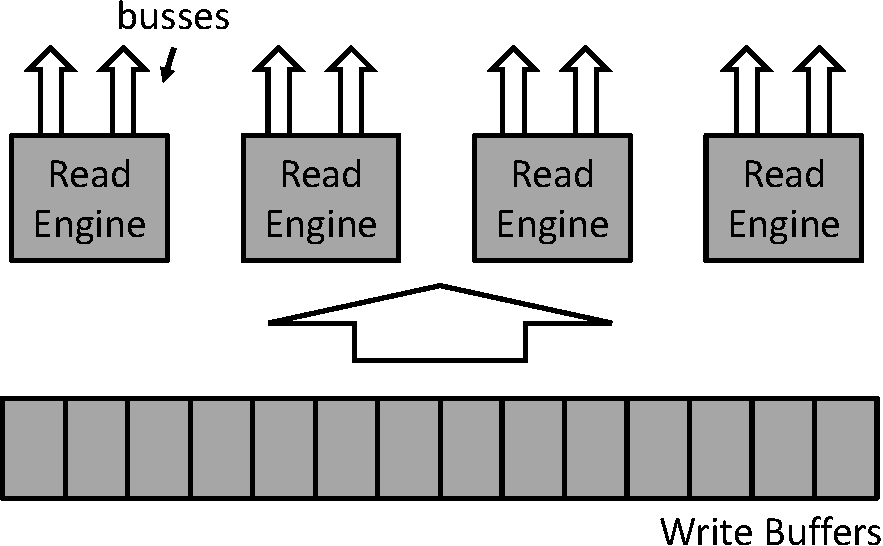
\includegraphics[width=0.23\textwidth]{figures/readinterface-crop.pdf}}
%	\subfloat[Reading Data from Storage]
%		{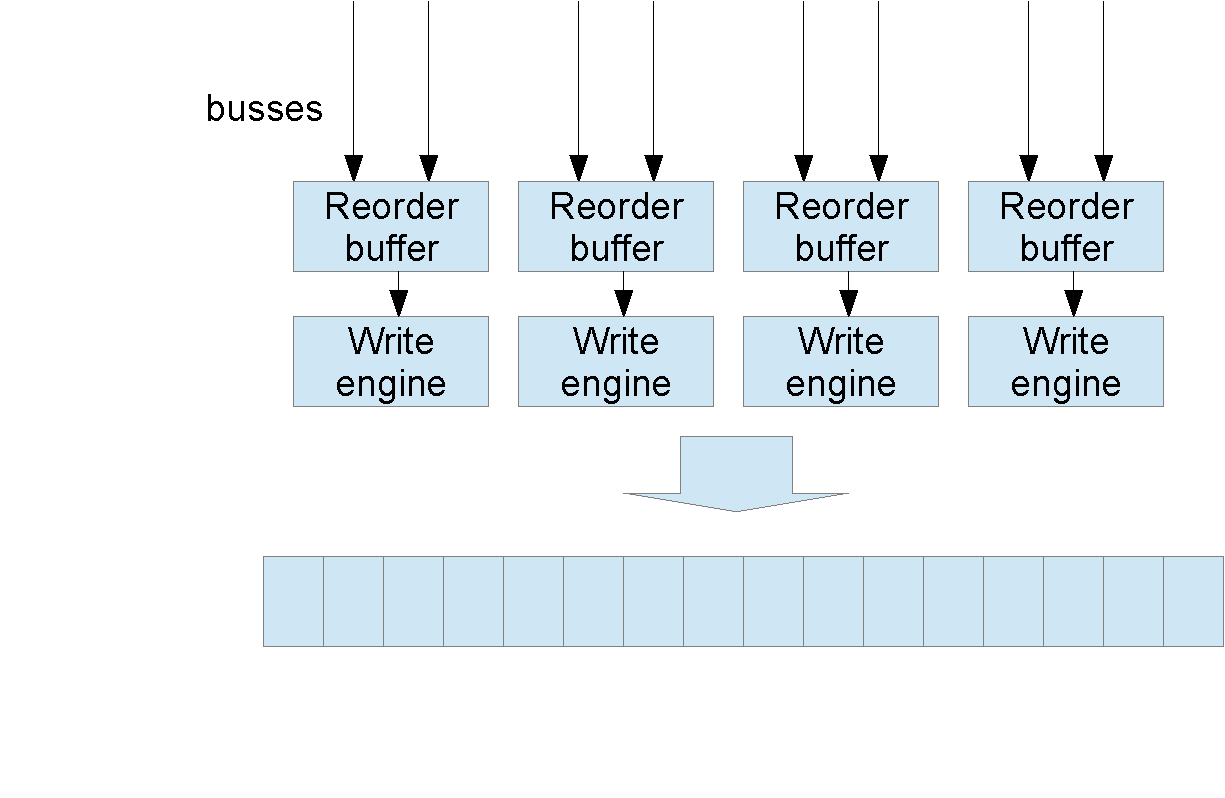
\includegraphics[width=0.23\textwidth]{figures/writeinterface-crop.pdf}}
	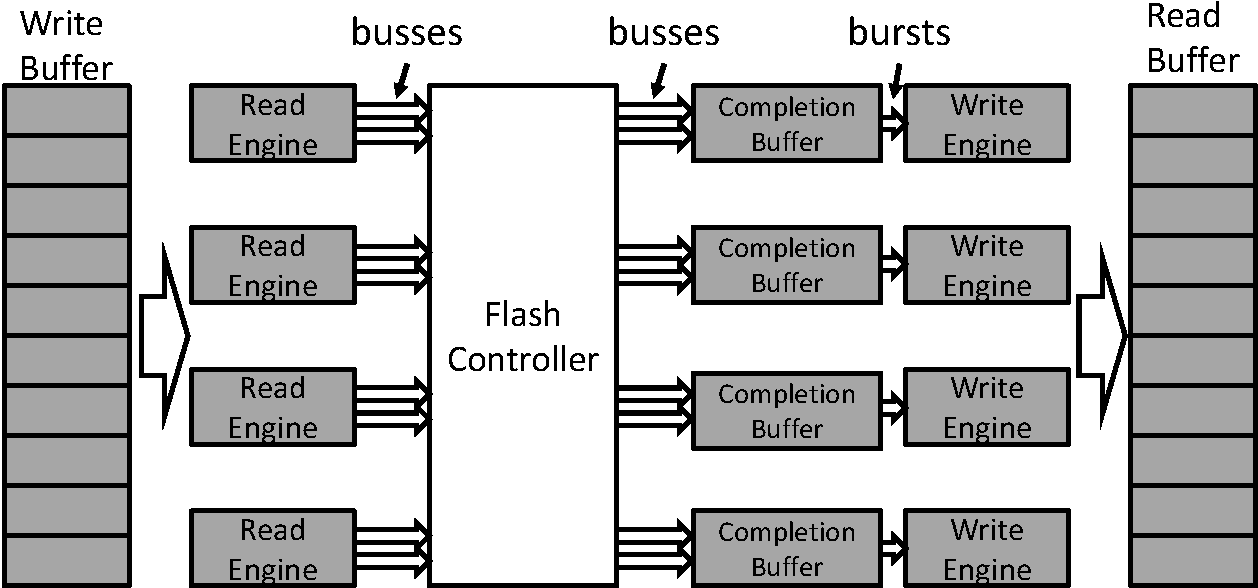
\includegraphics[width=0.4	\textwidth]{figures/hostinterface-crop.pdf}
	\caption{Host-FPGA Interface Over PCIe}
	\label{fig:hostinterface}
\end{figure}

%TODO: \subsubsection{Storage Bridge to Host}
